\chapter{Progettazione e Codifica}
\label{chap:design_coding}

In questo capitolo verranno descritti i processi di progettazione e codifica utilizzati nello sviluppo dell'applicazione \gls{ddcserviceg}\glox.
Si esamineranno l'architettura dell'applicazione, le tecnologie utilizzate per il \textit{frontend} e il \textit{backend}, i protocolli di comunicazione, l'autenticazione e l'architettura a componenti.

\section{\textit{Backend} e \textit{frontend}}
\label{subsec:backend_frontend}

In questa sezione, verranno descritti il \textit{backend} e il \textit{frontend} dell'applicazione \gls{ddcserviceg}\glox.
Si analizzeranno le differenze tra le due parti, le tecnologie utilizzate e le responsabilità di ciascuna componente.

\begin{figure}[H]
    \centering
    
\includegraphics[alt={Rappresentazione grafica delle tecnologie per backend e frontend}, height=5cm]{img/frontendbackend.png}
    \caption{Tecnologie utilizzate per {Frontend} e {Backend} di una \textit{app}}
    \label{fig:backendfrontend}
\end{figure}

\subsection{Responsabilità del \textit{backend}}
Il \textit{backend} dell'applicazione è scritto in \textit{Node.js} utilizzando \textit{TypeScript}, una scelta che combina la flessibilità e la velocità di \textit{Node.js} con la robustezza della tipizzazione statica di \textit{TypeScript}.
Il \textit{backend} ha diverse responsabilità cruciali:

\begin{itemize}
    \item \textbf{Gestione dei Dati}: Il \textit{backend} gestisce l'archiviazione, il recupero e la manipolazione dei dati.
    Utilizza diversi \textit{Database} per memorizzare informazioni strutturate.
    Inoltre, il \textit{backend} si interfaccia con servizi di \textit{cloud storage} come \textit{Amazon S3} di \textit{AWS} per memorizzare file e oggetti di grandi dimensioni, garantendo alta disponibilità e durabilità.
    \item \textbf{Autenticazione}: L'autenticazione degli utenti è un'altra responsabilità fondamentale del \textit{backend}.
    L'autenticazione gestita dal \textit{backend} offre un livello di sicurezza maggiore per diverse ragioni:
    \begin{itemize}
        \item \textbf{Controllo Centralizzato:} Il \textit{backend} funge da punto centrale per la verifica delle credenziali degli utenti, garantendo che tutti i tentativi di accesso siano gestiti in modo uniforme e sicuro.
        Questo riduce il rischio di inconsistenze e vulnerabilità che potrebbero sorgere se l'autenticazione fosse distribuita su più \textit{client}.
        \item \textbf{Protezione dei Segreti:} Nel \textit{backend}, è possibile mantenere i segreti e le chiavi di crittografia al sicuro, lontano dai dispositivi degli utenti dove potrebbero essere più facilmente compromessi.
        Ciò include la gestione sicura delle \textit{password}, che vengono memorizzate come \textit{hash} sicuri, e la generazione di \textit{token} di accesso.
        \item \textbf{Validazione e Scadenza dei Token:} Il \textit{backend} può gestire la generazione, la validazione e la scadenza dei \textit{token} di accesso \textit{JWT}, assicurando che solo i token validi e non scaduti possano essere utilizzati per accedere alle risorse protette.
        Questo meccanismo previene l'accesso non autorizzato e garantisce che gli utenti debbano autenticarsi periodicamente.
        \item \textbf{Log e Monitoraggio:} Il \textit{backend} può registrare tutte le attività di autenticazione, facilitando il monitoraggio e l'analisi dei tentativi di accesso.
        Questo aiuta a identificare e rispondere rapidamente a potenziali attacchi, come tentativi di forza bruta o accessi sospetti.
    \end{itemize}
    Questi vantaggi fanno sì che l'autenticazione gestita dal \textit{backend} sia un componente cruciale per la sicurezza complessiva dell'applicazione, proteggendo le informazioni sensibili degli utenti e garantendo l'integrità e la riservatezza dei dati.
    \item \textbf{Logica di Business}: Il \textit{backend} contiene la logica di business dell'applicazione, questa logica è separata in moduli e servizi, rendendo il codice più organizzato e manutenibile.
    I servizi nel \textit{backend} sono responsabili di eseguire operazioni come la validazione dei dati, l'elaborazione delle transazioni, e la comunicazione con servizi esterni.
    \item \textbf{API}: Il \textit{backend} espone \textit{API} REST e \textit{GraphQL} che permettono al \textit{frontend} di interagire con i dati e le funzionalità dell'applicazione. Le \textit{API REST} sono utilizzate per operazioni standard \textit{CRUD (Create, Read, Update, Delete)} e seguono una struttura basata su risorse. 
    \textit{GraphQL}, d'altra parte, offre una maggiore flessibilità permettendo al \textit{frontend} di specificare esattamente quali dati necessita, riducendo così il sovraccarico di rete e migliorando l'efficienza.
\end{itemize}

\subsection{Responsabilità del \textit{frontend}}
Il \textit{frontend} dell'applicazione è la parte visibile e interattiva che gli utenti utilizzano.
È sviluppato utilizzando \textit{Expo} e \textit{Next.js}, con \textit{Expo} destinato alle piattaforme \textit{mobile} e \textit{Next.js} alle piattaforme \textit{web}.
Il linguaggio di programmazione utilizzato per il \textit{frontend} è \textit{Typescript}. Le principali responsabilità del \textit{frontend} includono:
    \begin{itemize}
        \item \textbf{Interfaccia Utente (UI)}: Il \textit{frontend} è responsabile della presentazione visiva e dell'interazione dell'utente con l'applicazione.
        Utilizza componenti \textit{React} per costruire un'interfaccia modulare e riutilizzabile. Ogni componente rappresenta una parte della \textit{UI}, come bottoni, moduli di \textit{input}, e \textit{layout} di pagina.
        \item \textbf{Gestione dello Stato}: La gestione dello stato è un aspetto critico del \textit{frontend}. Utilizzando \textit{Redux}, una libreria per la gestione dello stato, l'applicazione mantiene uno stato globale che può essere condiviso tra vari componenti.
        \item \textbf{Interazione con le \textit{API}}: Il \textit{frontend} interagisce con il \textit{backend} attraverso le \textit{API REST} e \textit{GraphQL}. Utilizzando librerie come \textit{Axios} o \textit{Fetch}, il \textit{frontend} invia richieste \textit{HTTP} al \textit{backend} per recuperare, creare, aggiornare o eliminare dati.
        Le risposte del \textit{backend} sono quindi utilizzate per aggiornare l'interfaccia utente, rendendo i dati dinamicamente disponibili agli utenti.
        \item \textbf{Navigazione e Routing}: Il \textit{frontend} gestisce la navigazione tra le diverse pagine dell'applicazione, permettendo agli utenti di spostarsi fluidamente all'interno dell'interfaccia.
        Questo include la definizione di percorsi e la gestione delle transizioni tra le pagine, assicurando una suddivisione logica dell'applicazione in sezioni distinte e accessibili.
    \end{itemize}

\subsection{Differenze tra \textit{backend} e \textit{frontend}}
Sebbene il \textit{backend} e il \textit{frontend} siano strettamente collegati, essi hanno ruoli e responsabilità distinti:

\begin{itemize}
    \item \textbf{Tecnologie}: Il \textit{backend} è sviluppato in \textit{Node.js}, focalizzandosi sulla gestione dei dati, la logica di business e le \textit{API}. 
    Il \textit{frontend}, invece, è sviluppato utilizzando \textit{Expo} per le piattaforme \textit{mobile} e \textit{Next.js} per le piattaforme \textit{web}, concentrandosi sull'interfaccia utente e l'esperienza dell'utente.
    
    \item \textbf{Responsabilità}: 
    \begin{itemize}
        \item \textbf{Backend}: Gestisce la logica di business, l'autenticazione, la gestione dei dati e la comunicazione con i servizi esterni.
        \item \textbf{Frontend}: Si occupa della presentazione visiva, l'interazione dell'utente, la gestione dello stato e la navigazione.
    \end{itemize}

    \item \textbf{Interazione}: Il \textit{backend} e il \textit{frontend} comunicano tramite \textit{API}, dove il \textit{backend} fornisce i dati e le funzionalità necessarie, mentre il \textit{frontend} li utilizza per creare un'interfaccia utente interattiva e dinamica.
\end{itemize}

\subsection{Flusso di Lavoro Complessivo}
Il flusso di lavoro dell'applicazione prevede che l'utente interagisca con il \textit{frontend}, che a sua volta invia richieste al \textit{backend}. Il \textit{backend} elabora queste richieste, esegue la logica di business necessaria, interagisce con i \textit{database} e i servizi esterni, e infine restituisce una risposta al \textit{frontend}.
Il \textit{frontend} quindi aggiorna l'interfaccia utente in base alla risposta ricevuta, garantendo un'esperienza utente fluida e interattiva.
In sintesi, il \textit{backend} e il \textit{frontend} dell'applicazione \gls{ddcserviceg}\glox lavorano insieme per fornire un servizio completo ed efficiente, ognuno con ruoli e responsabilità specifici ma complementari.
Questa architettura modulare e separata permette di sviluppare, mantenere e scalare l'applicazione in modo efficace.


\subsection{Struttura delle Applicazioni}
\label{subsec:struttura_applicazioni}

La struttura complessiva delle applicazioni è organizzata in modo da mantenere il codice manutenibile e modulare.
Questo approccio consente di gestire facilmente la complessità del progetto, facilitando lo sviluppo, la collaborazione e la scalabilità. 
La disposizione delle \textit{directory} e dei file è progettata per riflettere la suddivisione logica delle funzionalità, garantendo che ogni componente del sistema sia isolato e riutilizzabile.


\subsection{Monorepo}
L'utilizzo di una \gls{monorepog}\glox è una strategia che permette di gestire tutto il codice del progetto in un unico \gls{repog}\glox.
Questo approccio offre numerosi vantaggi, tra cui:

\begin{itemize}
    \item \textbf{Condivisione del Codice}: Facilita la condivisione di moduli e librerie comuni tra diverse parti dell'applicazione, evitando duplicazioni e incoerenze.
    Questo approccio è particolarmente utile per il progetto \textit{DDC Service}, poiché consente di riutilizzare parti comuni tra l'applicazione \textit{DDC} e \textit{DDC Service}, come il \textit{Design System}, garantendo una coerenza visiva e funzionale tra le due applicazioni.
    \item \textbf{Gestione delle Dipendenze}: Permette di avere una gestione migliore delle dipendenze, semplificando l'aggiornamento e la sincronizzazione delle librerie utilizzate.
    Questo è essenziale per mantenere un ambiente di sviluppo stabile e aggiornato, riducendo i conflitti e le incompatibilità tra le diverse parti del progetto.
    \item \textbf{Collaborazione}: Migliora la collaborazione tra i \textit{team}, offrendo una visione unificata del progetto e facilitando la revisione del codice.
    I \textit{team} possono lavorare contemporaneamente su diverse parti dell'applicazione, beneficiando della trasparenza e della coerenza del codice condiviso.
    \item \textbf{Strumenti di Build e CI/CD}: Consente di configurare strumenti di build e \gls{cicdg}\glox in modo centralizzato, ottimizzando i processi di integrazione e distribuzione continua.
    Questo permette di automatizzare i test, il rilascio e il \textit{deploy} delle applicazioni \textit{DDC} e \textit{DDC Service}, assicurando che le nuove funzionalità e le correzioni di bug siano implementate rapidamente e senza intoppi.
\end{itemize}
Per questo progetto si è deciso di utilizzare la tecnologia \textit{monorepo} presente con \textit{npm workspaces}.
Questo primo approccio è stato scelto in quanto è stata la configurazione già addottata per \textit{DDC}, tuttavia, come verrà analizzato nel capitolo successivo, ci sono soluzioni migliore.

\pagebreak
\subsubsection{Struttura delle \textit{directory}}
\label{subsec:strutturadirectory}

La struttura del progetto è organizzata come segue:
{\tiny\dirtree{%
.1 root.
.2 apps. 
.3 ddc-service-expo.
.4 android \hspace{5em} (Build Android).
.4 ios \hspace{5em} (Build IOS).
.4 public.
.4 app \hspace{5em} (Routing e Navigazione).
.4 app.json.
.4 index.json.
.4 tsconfig.json.
.4 package.json.
.4 node\_modules.
.3 ddc-service-next.
.4 pages \hspace{2em} (Routing e Navigazione).
.4 public.
.4 package.json.
.4 node\_modules.
.4 tsconfig.json.
.3 expo \hspace{2em} (App DDC).
.3 next \hspace{2em} (App DDC).
.2 packages.
.3 app \hspace{2em} (App \textit{DDC}).
.3 \textit{DDC}-service  \hspace{2em} (App \textit{DDC Service}).
.4 components.
.4 features.
.4 provider.
.4 store.
.4 utils.
.4 package.json.
.4 node\_modules.
.3 design-system. 
.3 hooks.
.3 utils.
.2 scripts.
.2 tsconfig.json.
.2 .gitignore.
.2 package.json.
.2 node\_modules.
}}

\pagebreak
\subsection{Visione Generale}
La struttura del progetto è organizzata per supportare lo sviluppo e la gestione di quattro applicazioni principali: 
due applicazioni \textit{DDC} (una per \textit{Expo} e una per \textit{Next}) e due applicazioni \textit{DDC Service} (una per \textit{Expo} e una per \textit{Next}).
La suddivisione in diverse \textit{directory} facilita la condivisione del codice, delle risorse e delle configurazioni tra le applicazioni, migliorando la manutenibilità e la modularità del progetto.
\footcite{site:monorepomigration}

Le \textit{directory} principali sono suddivise come segue:
\begin{itemize}
    \item \textbf{apps}: Contiene le applicazioni specifiche per \textit{DDC} e \textit{DDC Service}. 
    Ogni applicazione ha una \textit{directory} separata per le versioni \textit{Expo} e \textit{Next}.
    Le applicazioni contenute qui sono la struttura portante rispettivamente di \textit{Next} ed \textit{Expo}, e il codice contenuto dentro queste cartelle si occupa solamente di navigazione e \textit{routing}.
    \item \textbf{packages}: Contiene le applicazioni ma anche i pacchetti condivisi tra le applicazioni, inclusi componenti, \textit{utils, hooks} e il \textit{Design System}.
    il package \textit{utils} contiene funzioni utili per tutte le applicazioni che possono essere riutilizzate in ambito sviluppo multipiattaforma.
    \item \textbf{scripts}: Contiene \textit{script} per automatizzare varie attività di sviluppo e di \textit{deployment}.
    \item \textbf{Configurazioni}: File di configurazione globali, come \textit{tsconfig.json}, \textit{package.json} e \textit{.gitignore}.
\end{itemize}

\subsection{Descrizione delle \textit{directory}}
\begin{itemize}
    \item \textbf{apps}
    La \textit{directory} \texttt{apps} contiene le applicazioni specifiche per \textit{DDC} e \textit{DDC Service}, organizzate come segue:
    \begin{itemize}
        \item \textbf{ddc-service-expo}: Contiene la versione \textit{Expo} dell'applicazione \textit{DDC Service}. Include le \textit{directory} per Android e iOS, oltre a file di configurazione specifici per \textit{Expo}.
        \item \textbf{ddc-service-next}: Contiene la versione \textit{Next} dell'applicazione \textit{DDC Service}. Include le pagine dell'applicazione e i file di configurazione specifici per \textit{Next.js}.
        \item \textbf{expo (DDC)}: Contiene la versione \textit{Expo} dell'applicazione \textit{DDC}.
        \item \textbf{next (DDC)}: Contiene la versione \textit{Next} dell'applicazione \textit{DDC}.
    \end{itemize}

    \item \textbf{packages}
    La \textit{directory} \texttt{packages} contiene i pacchetti condivisi tra le applicazioni, organizzati come segue:
    \begin{itemize}
        \item \textbf{app}: Pacchetto contenente le applicazioni e le pagine condivise tra le versioni \textit{Expo} e \textit{Next} dell'applicazione \textit{DDC}.
        \item \textbf{ddc-service}: Pacchetto contenente componenti, funzionalità, provider, \textit{store} e utilità specifici per l'applicazione \textit{DDC Service}.
        \item \textbf{design-system}: Pacchetto contenente il \textit{Design System} condiviso tra le applicazioni, incluso il tema dell'applicazione e i componenti di base.
        \item \textbf{hooks}: Pacchetto contenente \textit{hook} condivisi tra le applicazioni.
        \item \textbf{utils}: Pacchetto contenente utilità condivise tra le applicazioni.
    \end{itemize}

    \item \textbf{scripts}
    La \textit{directory} \texttt{scripts} contiene script per automatizzare varie attività di sviluppo, come l'installazione delle dipendenze, la costruzione e il deployment delle applicazioni.

    \item \textbf{Configurazioni}
    Nella root del progetto si trovano vari file di configurazione globali, tra cui:
    \begin{itemize}
        \item \texttt{postinstall.json}: Script eseguiti dopo l'installazione delle dipendenze.
        \item \texttt{tsconfig.json}: Configurazione \textit{Typescript} condivisa tra tutte le applicazioni e i pacchetti.
        \item \texttt{.gitignore}: File che specifica i file e le \textit{directory} da ignorare nel controllo di versione.
        \item \texttt{package.json}: Gestione delle dipendenze e script di progetto.
        \item \texttt{node\_modules}: \textit{directory} generata automaticamente che contiene tutte le dipendenze installate.
    \end{itemize}
\end{itemize}

\subsection{Gestione delle Dipendenze}
All'interno del file \textit{package.json} situato nella \textit{root} del progetto, sono configurati diversi parametri che definiscono la struttura della \textit{monorepo}. 
In particolare, c'è una suddivisione tra due principali categorie di \textit{workspaces}: \textit{apps} e \textit{packages}.
Per \textit{workspace} ci si riferisce alle cartelle contenute all'interno delle \textit{directory} \textit{apps} e \textit{packages}.
Ad esempio, \textit{ddc-service-expo} è considerato un \textit{workspace}.
\\Questa suddivisione permette una gestione organizzata e modulare del codice, facilitando la manutenzione e la scalabilità del progetto.
Per quanto riguarda la gestione delle dipendenze, quando si utilizza un \textit{package} esterno, è necessario installarlo nel corretto \textit{workspace}. 
Ogni \textit{workspace} ha il proprio file \textit{package.json}, che contiene solo le dipendenze specifiche necessarie per quel \textit{workspace}.
Questa separazione garantisce che ogni parte del progetto abbia accesso solo alle librerie di cui ha bisogno, evitando conflitti e riducendo il rischio di dipendenze non utilizzate.
Inoltre, ogni \textit{workspace} ha una propria cartella \textit{node\_modules} dedicata, che contiene tutte le librerie e le dipendenze installate specificamente per quel \textit{workspace}.
Questa configurazione consente di mantenere un ambiente di sviluppo isolato per ciascun \textit{workspace}, facilitando la gestione e l'aggiornamento delle dipendenze in modo indipendente.
In sintesi, l'uso di \textit{workspaces} e la gestione decentralizzata delle dipendenze attraverso file \textit{package.json} separati e cartelle \textit{node\_modules} dedicate contribuiscono a rendere la \textit{monorepo} più organizzata, modulare e manutenibile.
Questa struttura permette ai \textit{team} di sviluppo di lavorare in modo più efficiente, riducendo i tempi di integrazione e semplificando il processo di aggiornamento delle librerie.
\footcite{site:monorepomigration}
\pagebreak

\section{Comunicazione}
\label{sec:comunicazione}

La comunicazione tra il \textit{frontend} e il \textit{backend} è un aspetto cruciale nello sviluppo di applicazioni moderne.
Questo capitolo descrive i protocolli di comunicazione utilizzati, come \textit{REST e \textit{GraphQL}}, e l'uso di strumenti di \textit{code generation} per mantenere il codice tipizzato e sincronizzato con lo schema \textit{GraphQL}.

\subsection{Protocolli di Comunicazione}
\label{subsec:protocolli_comunicazione}

Per garantire una comunicazione efficace e sicura tra il \textit{frontend} e il \textit{backend}, sono stati adottati diversi protocolli di comunicazione.
Tra i principali protocolli utilizzati troviamo \textit{REST e \textit{GraphQL}}, ciascuno con specifici casi d'uso e vantaggi.

\begin{figure}[H]
    \centering
    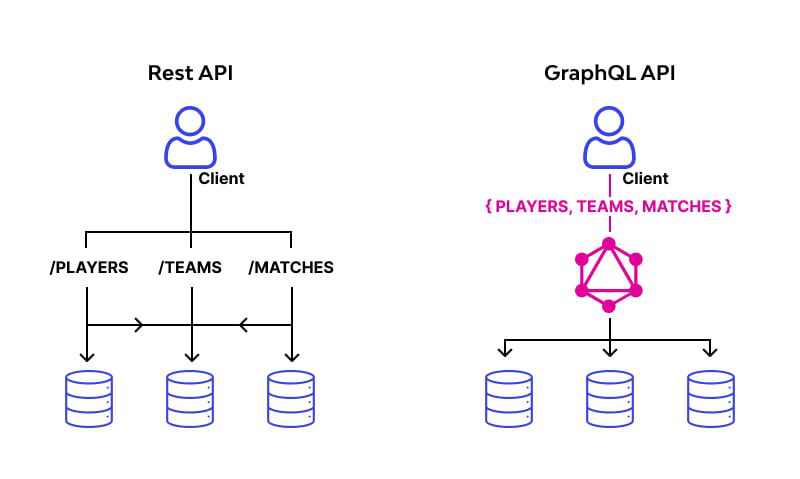
\includegraphics[alt={Rappresentazione grafica della struttura e differenza tra rest api e graphqlapi}, height=5cm]{img/restgraphql.png}
    \caption{Rest API vs GraphQL API}
    \label{fig:restapivsgraphqlapi}
\end{figure}

\subsubsection{REST}
La \textit{API REST} è stata utilizzata principalmente per l'autenticazione degli utenti.
\textit{REST} è un'architettura leggera che utilizza i metodi \textit{HTTP standard (GET, POST, PUT, DELETE)} per eseguire operazioni \textit{CRUD (Create, Read, Update, Delete)} sui dati.
Un esempio di \textit{endpoint REST} per l'autenticazione potrebbe essere:
\begin{verbatim}
POST /api/auth/login
{
    "username": "example_user",
    "password": "example_password"
}
\end{verbatim}

Questo \textit{endpoint} accetta le credenziali dell'utente e, se valide, restituisce un \gls{jwt}\glox che viene utilizzato per autenticare le richieste successive.

\subsubsection{GraphQL}
\textit{GraphQL} è un linguaggio di \textit{query} per le \textit{API} che offre una maggiore flessibilità rispetto a \textit{REST}.
In \textit{DDC Service}, una volta ottenuto il \textit{token JWT} tramite \textit{REST}, \textit{GraphQL} viene utilizzato per interrogare il \textit{backend}.
I vantaggi di \textit{GraphQL} includono la possibilità di richiedere esattamente i dati necessari e la riduzione del numero di richieste necessarie per ottenere tutte le informazioni richieste.

Esempio generico di una \textit{query} \textit{GraphQL}:
\begin{verbatim}
query {
    user(id: "123") {
        id
        name
        email
    }
}
\end{verbatim}

Esempio generico di una mutazione \textit{GraphQL}:
\begin{verbatim}
mutation {
    updateUser(id: "123", input: {name: "New Name"}) {
        id
        name
        email
    }
}
\end{verbatim}

\textit{GraphQL} è stato scelto per la sua efficienza nella gestione delle richieste complesse e per la sua capacità di evolversi senza influenzare le versioni precedenti dell'\textit{API}.

\subsection{GraphQL Codegen e RTK \textit{query}}
\label{subsec:graphql_codegen}

L'utilizzo combinato di strumenti di \textit{code generation} per \textit{GraphQL}, come \textit{GraphQL Code Generator}, e \gls{rtkg}\glox è fondamentale per mantenere il codice tipizzato e sincronizzato con lo schema \textit{GraphQL}.
\textit{GraphQL Code Generator} genera automaticamente tipi \textit{Typescript} per le \textit{query}, le mutazioni e i frammenti definiti, mentre \textit{RTK query} facilita l'integrazione di queste \textit{query} nel sistema di gestione dello stato.
Questa combinazione migliora la sicurezza del tipo e riduce gli errori di \textit{runtime}, oltre a fornire un'architettura chiara e scalabile per la gestione delle \textit{API} \textit{GraphQL} nel \textit{frontend}.

\subsubsection{Configurazione e Utilizzo}
La configurazione di \textit{GraphQL Codegen} nel progetto è semplice e diretta. I file \textit{.graphql}, contenenti tutte le \textit{query} da eseguire, sono memorizzati all'interno della cartella \textit{graphql/documents}.

Di seguito è riportato un esempio di configurazione nel file \textit{codegen.config.ts}:

\begin{listing}[H]
    \begin{minted}{typescript}
    import { CodegenConfig } from '@graphql-codegen/cli'

    const config: CodegenConfig = {
    schema: './store/graphql/schema.json',
    documents: ['./store/graphql/documents/**/*.graphql'],
    ignoreNoDocuments: true, // for better experience with the watcher
    generates: {
        './store/graphql/queryBaseApi.ts': {
        plugins: [
            'typescript',
            'typescript-operations',
            'typescript-resolvers',
            {
            'typescript-rtk-query': {
                importBaseApiFrom: 'ddc-service/store/api/baseApi',
                importBaseApiAlternateName: 'baseApi',
                exportHooks: true,
            },
            },
        ],
        },
    },
    }

    export default config
    \end{minted}
    \caption{Configurazione \textit{GraphQL Codegen: codegen.config.ts}}
    \label{listing_confgraphql_codegen}
\end{listing}

Questo file di configurazione specifica l'endpoint dello schema \textit{GraphQL} (\textit{schema.json}), 
i documenti \textit{GraphQL} (\textit{documents}) da cui generare il codice, e i plugin da utilizzare per la generazione.
Inoltre, viene generato un file chiamato \textit{queryBaseApi.ts}, che contiene tutte le \textit{query} e le mutazioni definite nei file \textit{.graphql}.

Una volta configurato, è possibile eseguire il comando di generazione:

\begin{verbatim}
graphql-codegen
\end{verbatim}

Il file \textit{queryBaseApi.ts} generato viene utilizzato per integrare le \textit{query} e le mutazioni \textit{GraphQL} nel codice del \textit{frontend}, sfruttando \textit{Redux} per la gestione della \textit{cache}.

Queste \textit{API} sono cachate su \textit{Redux} e possono essere chiamate semplicemente con:

\begin{listing}[H]
    \begin{minted}{typescript}
        import { useGetOvensQuery } 
        from 'ddc-service/store/graphql/queryBaseApi'
    \end{minted}
    Per utilizzare la \textit{query}:
    \begin{minted}{typescript}
        const { data, isFetching, isLoading, isSuccess, 
        isError, isUninitialized, error, refetch } = useGetOvensQuery({})
    \end{minted}
    \caption{Utilizzo \textit{API} \textit{GraphQL}}
    \label{listing_utilizzo_api}
\end{listing}

\begin{itemize}
  \item \textbf{data}: contiene i dati recuperati dalla \textit{query}.
  \item \textbf{isFetching}: booleano che indica se la \textit{query} è attualmente in fase di recupero.
  \item \textbf{isLoading}: booleano che indica se la \textit{query} è in fase di caricamento iniziale.
  \item \textbf{isSuccess}: booleano che indica se la \textit{query} è stata completata con successo.
  \item \textbf{isError}: booleano che indica se c'è stato un errore nell'esecuzione della \textit{query}.
  \item \textbf{isUninitialized}: booleano che indica se la \textit{query} non è stata ancora eseguita.
  \item \textbf{error}: contiene informazioni sull'errore se la \textit{query} ha fallito.
  \item \textbf{refetch}: funzione che permette di eseguire nuovamente la \textit{query}.
\end{itemize}

L'utilizzo di \textit{GraphQL Codegen} garantisce che il codice rimanga sincronizzato con lo schema \textit{GraphQL}, 
riducendo il rischio di errori e migliorando la produttività del \textit{team} di sviluppo.





\subsection{Autenticazione}
\label{subsec:autenticazione}

Il sistema di autenticazione utilizzato nell'applicazione è cruciale per garantire che solo gli utenti autorizzati possano accedere ai dati e alle funzionalità disponibili.
Questo sistema si basa su flussi di autenticazione ben definiti, utilizza \gls{jwtg}\glox e implementa diverse strategie di sicurezza per mantenere l'integrità e la riservatezza dei dati.

\subsubsection{Backend Stateless}
Un \textit{backend stateless} è un'architettura in cui il \textit{server} non mantiene alcuna informazione di stato tra le richieste dei \textit{client}.
Ogni richiesta che arriva al \textit{server} deve contenere tutte le informazioni necessarie per essere processata.
Questo approccio offre diversi vantaggi, tra cui:

\begin{itemize}
    \item \textbf{Scalabilità}: Poiché il \textit{server} non deve mantenere informazioni di stato, può facilmente scalare orizzontalmente aggiungendo più istanze per gestire un numero maggiore di richieste.
    \item \textbf{Resilienza}: Se un \textit{server} va \textit{offline}, le richieste possono essere indirizzate a un altro \textit{server} senza perdere dati di sessione.
    \item \textbf{Semplicità}: La gestione delle sessioni non è necessaria, riducendo la complessità del codice del \textit{server}.
\end{itemize}

Nel contesto di questo progetto, il \textit{backend} è ospitato su \textit{AWS}, utilizzando vari servizi cloud per garantire affidabilità e scalabilità.

\subsubsection{Flussi di Autenticazione}
I flussi di autenticazione principali includono \textit{login}, registrazione e recupero della \textit{password}.
Durante il \textit{login}, il \textit{frontend} invia le credenziali dell'utente al \textit{backend} tramite un \textit{endpoint REST}.
Il \textit{backend} verifica le credenziali e, se valide, genera un \textit{token JWT} che viene inviato al \textit{frontend} per essere utilizzato nelle richieste successive. 
Nel caso della registrazione, l'utente fornisce le informazioni necessarie, che vengono inviate al \textit{backend}.
Il \textit{backend} crea un nuovo utente nel database e, se la registrazione è avvenuta con successo, restituisce un token JWT al \textit{frontend}.
Per il recupero della password, l'utente invia una richiesta di \textit{reset} tramite un \textit{endpoint REST}.
Il \textit{backend} genera un link di recupero della password e lo invia all'indirizzo email dell'utente.
L'utente può quindi utilizzare questo \textit{link} per reimpostare la propria \textit{password}.

\subsubsection{Gestione Cookie}
Inizialmente, il \textit{backend} utilizzava \textit{Passport} per gestire le sessioni in modalità \textit{stateless}, 
il che significa che non memorizza informazioni sulla sessione degli utenti tra le richieste.
In questo approccio, i cookie venivano inviati al client con il comando \textit{Set-Cookie}, e il \textit{client} era responsabile di memorizzare e inviare i \textit{cookie} contenenti le sessioni e le firme con ogni richiesta successiva.
Tuttavia, la gestione dei \textit{cookie} su piattaforme native come \textit{Android} e \textit{IOS} ha presentato delle sfide.
Ad un primo sguardo può sembrare impossibile avere i \textit{cookie} su piattaforme native, e gli si considera solo per il \textit{web}.
In verità \textit{React Native} e la sua libreria \textit{fetch} integrata hanno un'implementazione nativa dei \textit{cookie}.
Questa implementazione nativa innanzitutto diferisce in base alla piattaforma, tra \textit{IOS e Android}, e ha diverse politiche di gestione
rispetto al browser, per esempio la gestione differisce nelle politiche \textit{CORS}.
Inoltre, la gestione dei \textit{cookie} su dispositivi mobili richiede l'uso di librerie di gestione dei \textit{cookie} e non può essere effettuata tramite semplici richieste \textit{HTTP} come avviene nei browser. 
Queste limitazioni hanno reso chiaro che, pur essendo possibile, un sistema di autenticazione basato sui cookie per piattaforme native non è praticabile.
\footcite{site:reactnativecookieauth}

\subsubsection{Gestione dei Token JWT}
A causa delle problematiche riscontrate con i cookie, è stato deciso di adottare i JSON \textit{web} Tokens (JWT) per l'autenticazione. 
I JWT sono token compatti, URL-safe, che rappresentano in modo sicuro le informazioni tra due parti.
Un token JWT è composto da tre parti: header, payload e signature.

\begin{itemize}
    \item \textbf{Header}: Contiene il tipo di token (JWT) e l'algoritmo di firma (es. HMAC SHA256).
    \item \textbf{Payload}: Contiene le informazioni dell'utente (claims), come l'ID utente e le autorizzazioni.
    \item \textbf{Signature}: Viene creata utilizzando l'algoritmo specificato nell'header e una chiave segreta. Serve a verificare che il token non sia stato modificato.
\end{itemize}

I JWT sono sicuri perché la firma digitale impedisce la manipolazione dei dati contenuti nel token.
Inoltre, essi funzionano bene con un \textit{backend} stateless, poiché tutte le informazioni necessarie per autenticare una richiesta sono contenute nel token stesso.
Questo elimina la necessità di mantenere sessioni sul \textit{server}, migliorando la scalabilità e riducendo il carico sul \textit{backend}.
In conclusione, l'adozione dei JWT per l'autenticazione ha migliorato la sicurezza e l'efficienza dell'applicazione, risolvendo le problematiche di gestione dei cookie su piattaforme mobili e supportando un'architettura \textit{backend} stateless.

\section{Architettura a Componenti}
\label{sec:architettura_componenti}

\subsection{Componenti di Base \textit{Design System}}
I componenti di base dell'applicazione sono gli elementi fondamentali utilizzati per costruire l'interfaccia utente.
Questi componenti sono creati utilizzando \textit{React} e fanno parte del \textit{Design System}, un insieme di linee guida e componenti riutilizzabili che garantiscono coerenza e usabilità nell'applicazione.

Esempi di componenti di base includono \textit{Button}, \textit{input}, \textit{Text}, etc... 
Di seguito è riportato un esempio di un componente \textit{Text} a scopo dimostrativo:


\begin{listing}[H]
    \begin{minted}{typescript}
import React from 'react';
import { Text as RNText, TextProps } from 'dripsy';
import { useTheme } from '../Theme';

const Text = ({ style, ...props }: TextProps) => {
  const { colors } = useTheme();
  return <RNText style={[{ color: colors.text }, style]} {...props} />;
};

export default Text;
    \end{minted}
    \caption{Esempio Componente Text \textit{Design System}}
    \label{listing_text_design_system}
\end{listing}
Il codice sopra è solo un esempio di come potrebbe essere implementato un componente di base.
Un componente di base è un componente astratto che include solo funzionalità dedicate a se stesso,
senza logica legata all'architettura dell'applicazione.
Ad esempio, un componente del \textit{Design System} dedicato a elementi di \textit{layout} o a elementi comuni dell'interfaccia utente dell'applicazione è un componente di base.
Un errore comune nella realizzazione di componenti di base del \textit{Design System} è introdurre logica specifica dell'applicazione, 
come la gestione degli stati tramite \textit{Redux}.
Questa pratica lega la logica dell'applicazione ai componenti di base, rendendoli non riutilizzabili in futuro.
I componenti di base dovrebbero essere il più astratti possibile, gestendo la propria logica internamente e ricevendo i parametri di \textit{input} come props.
Se progettati correttamente, questi componenti possono essere utilizzati in diverse parti dell'applicazione senza dipendere da contesti specifici.
Per esempio, se un componente di base del \textit{Design System} viene utilizzato in una funzionalità dell'applicazione, ci si aspetta che possa essere riutilizzato anche in altre funzionalità senza modifiche.
Questi componenti devono seguire le linee guida del \textit{Design System} e le librerie grafiche comuni, ma devono rimanere indipendenti dalla logica specifica dell'applicazione.
Seguendo queste linee guida, i componenti di base possono essere progettati in modo da essere riutilizzabili, mantenibili e indipendenti dalla logica dell'applicazione, contribuendo così a un codice più pulito e modulare.

\subsection{Componenti Compositi}
I componenti compositi combinano i componenti di base per formare parti più complesse dell'interfaccia utente.
Ad esempio, un componente \textit{Form} potrebbe combinare vari \textit{input} e bottoni per creare un modulo di inserimento dati.

Questi componenti compositi sono spesso legati a singole funzionalità dell'applicazione e sono costruiti utilizzando i componenti di base del \textit{Design System}. 
La gestione gerarchica dei componenti in \textit{React} segue il pattern MVVM (Model-View-ViewModel), dove:

\begin{itemize}
    \item \textbf{Model}: rappresenta i dati dell'applicazione.
    \item \textbf{View}: rappresenta l'interfaccia utente e mostra i dati del Model.
    \item \textbf{ViewModel}: gestisce la logica di presentazione e l'interazione tra la View e il Model.
\end{itemize}

In \textit{React}, i componenti della View sono implementati come componenti funzionali o classi, 
mentre il \textit{ViewModel} può essere rappresentato da hook personalizzati o dallo stato locale dei componenti.
Questo approccio è particolarmente utile in ambito native perché consente una gestione modulare e riutilizzabile dell'interfaccia utente.

Ecco un esempio di componente composito TitleSection che combina componenti di base del \textit{Design System}:


\begin{listing}[H]
    \begin{minted}{typescript} 
import Button, { ButtonProps } 
    from '@unox/design-system/src/components/Button'
import { View } from 'dripsy'
import { isWebPlatform, useIsMobile } from '@unox/utils/breakpoints'
import Text from '@unox/design-system/src/components/Text'

const TitleSection = (props: {
    title?: string
    size: 'small' | 'large'
    textAlignCenter?: boolean
    subtitle?: string
    backgroundColor?: string
    button?: { showOnDesktop?: boolean; buttonProps: ButtonProps }
    secondButton?: { showOnDesktop?: boolean; buttonProps: ButtonProps }
    }) => {
    const { size, title, textAlignCenter, 
        subtitle, button, secondButton, backgroundColor } = props
    const isMobile = useIsMobile()
    const isSmall = size === 'small'
    const isLarge = size === 'large'

    return (/**/)
    //
}
    \end{minted}
    \caption{Esempio Componente TitleSection \textit{DDC Service}}
    \label{listing_titlesection_ddcservice}
\end{listing}
In questo esempio, si può vedere come i componenti \textit{Button, View e Text} vengano combinati per creare un nuovo componente composito.
I componenti compositi uniscono componenti di base per formare parti più complesse dell'interfaccia utente.
Questi componenti sono progettati per supportare funzionalità specifiche dell'applicazione, integrando spesso la logica necessaria per realizzare tali funzionalità.
I componenti compositi prendono componenti di base dal \textit{Design System} e li combinano per creare strutture più articolate come moduli, card o sezioni di \textit{layout}.
Questo approccio consente di costruire interfacce utente modulari e riutilizzabili, mantenendo il codice organizzato e facile da gestire.

\subsection{Esempi di Componenti Compositi}

In questa sezione verranno mostrati due esempi di componenti compositi.
Verranno mostrati solo gli import di questi componenti, in quanto già da qui si possono capire le funzionalità dei componenti e la loro struttura.

\subsubsection{SignInForm}

\begin{listing}[H]
    \begin{minted}{typescript} 
import { useSx, View } from 'dripsy'
import { Button } from '@unox/design-system/'
import { Text } from '@unox/design-system/'
import InputField from '@unox/design-system/src/components/InputField'
import { useRouter } from 'solito/router'
import useAuth from '../useAuth'
import { TextLink } from 'solito/link'
import useStylesByVariants from '@unox/hooks/useStylesByVariants'
import { RootState } from 'ddc-service/store'
import { useSelector } from 'react-redux'
import { useEffect, useState } from 'react'
const SignInForm = () => {
    const [email, setEmail] = useState('')
    const [password, setPassword] = useState('')
    const { authSignIn } = useAuth()
    const AUTH_SIGNIN_ERROR = 
        useSelector((state: RootState) => state.auth.AUTH_SIGNIN_ERROR)
    const { push, replace, back, parseNextPath } = useRouter()
    const errorModal = useErrorModal()
    const sx = useSx()
    const getStylesByVariants = useStylesByVariants()
    const recoverStyle = getStylesByVariants([['text.linkSmall']])
    const callBackSignIn = () => {
        authSignIn({ email, password })
    }
    return (/**/)
}
    \end{minted}
    \caption{Esempio Componente SignInForm \textit{DDC} Sercive}
    \label{listing_signinform_ddcservice}
\end{listing}


Il componente \texttt{SignInForm} è un modulo di autenticazione che permette agli utenti di accedere all'applicazione inserendo le proprie credenziali.
Analizziamo gli import per capire come è strutturato e quali funzionalità implementa:

\begin{itemize}
    \item \textbf{Layout e Stile}
    \begin{itemize}
        \item \texttt{useSx, View} da \texttt{dripsy}: \textit{Dripsy} è una libreria per la gestione degli stili in \textit{React} Native, particolarmente utile per applicazioni \textit{cross-platform}. \texttt{useSx} viene utilizzato per definire stili inline, mentre \texttt{View} è un contenitore per \textit{layout}.
        \item \texttt{useStylesByVariants} da \texttt{@unox/hooks/useStylesByVariants}: Questo hook permette di gestire varianti di stili, rendendo più facile applicare stili diversi in base a determinate condizioni.
    \end{itemize}
    
    \item \textbf{Componenti di Base del \textit{Design System}}
    \begin{itemize}
        \item \texttt{Button, Text} da \texttt{@unox/design-system/}: Sono componenti di base per i pulsanti e il testo, forniti dal \textit{Design System} dell'applicazione.
        \item \texttt{InputField} da \texttt{@unox/design-system/src/components/InputField}: Un campo di \textit{input} personalizzato, anch'esso parte del \textit{Design System}, utilizzato per raccogliere dati dagli utenti.
    \end{itemize}
    
    \item \textbf{Navigazione}
    \begin{itemize}
        \item \texttt{useRouter} da \texttt{solito/router}: Un hook per gestire la navigazione all'interno dell'applicazione. \texttt{push}, \texttt{replace}, \texttt{back} e \texttt{parseNextPath} sono metodi per la gestione delle rotte.
        \item \texttt{TextLink} da \texttt{solito/link}: Un componente per creare link testuali che permettono di navigare all'interno dell'applicazione.
    \end{itemize}
    
    \item \textbf{Autenticazione}
    \begin{itemize}
        \item \texttt{useAuth} da \texttt{../useAuth}: Un \textit{hook} personalizzato per gestire l'autenticazione, contiene funzioni per il \textit{login, logout} e altre operazioni correlate.
    \end{itemize}
    
    \item \textbf{Gestione dello Stato}
    \begin{itemize}
        \item \texttt{RootState} da \texttt{ddc-service/store}: Importa la definizione dello stato globale dell'applicazione gestito con \textit{Redux}.
        \item \texttt{useSelector} da \texttt{react-redux}: Un \textit{hook} per accedere al stato \textit{Redux}. In questo caso, viene utilizzato per ottenere l'errore di autenticazione (\texttt{AUTH\_SIGNIN\_ERROR}).
    \end{itemize}
    
    \item \textbf{Effetti e Stato Locale}
    \begin{itemize}
        \item \texttt{useEffect, useState} da \texttt{react}: \textit{Hook} per gestire gli effetti collaterali (\texttt{useEffect}) e lo stato locale (\texttt{useState}) del componente. \texttt{useState} viene utilizzato per gestire gli \textit{input} dell'email e della \textit{password}.
    \end{itemize}
    
    \item \textbf{Gestione degli Errori}
    \begin{itemize}
        \item \texttt{useErrorModal} \textit{Hook} per gestire e visualizzare errori tramite un \textit{modal}.
    \end{itemize}
\end{itemize}

\textbf{Scopo del Componente}

Il componente \textit{SignInForm} è progettato per gestire il processo di accesso degli utenti.
Gli utenti inseriscono le loro credenziali (email e password) nei campi di \textit{input}.
Quando l'utente preme il pulsante di accesso, la funzione \textit{authSignIn} viene chiamata, utilizzando i dati di stato locali per tentare l'autenticazione.
Il componente gestisce anche gli errori di autenticazione tramite \textit{Redux} e permette di visualizzare un messaggio di errore e un modal se l'autenticazione fallisce.
Inoltre, utilizza il \textit{router} per navigare tra le schermate in base ai risultati dell'autenticazione.


\subsubsection{ProductScreen}

\begin{listing}[H]
    \begin{minted}{typescript} 
import { useGetOvensQuery, useGetProductDetailsQuery, useSearchProductQuery,
} from 'ddc-service/store/graphql/queryBaseApi'
import { RefreshControl } from 'react-native'
import { View, H1, ScrollView } from 'dripsy'
import { createParam } from 'solito'
import { useRouter } from 'solito/router'
import Breadcrumbs, { BreadcrumpsCtrl } from '../../components/Breadcrumbs'
import { isWebPlatform, useIsDesktop, useIsLargeDesktop, useIsMobile, useIsSmallDesktop, useIsTablet,
} from '@unox/utils/breakpoints'
import { SearchBanner } from '../../components/SearchBanner'
import TechnicalSpecsBand from './components/TechnicalSpecsBand'
import DownlaodArea from './components/DownloadArea'
import ItemSummaryCard from './components/ItemSummaryCard'
import ContentCTA from './components/ContentCTA'
import { usePathname } from 'solito/navigation'
import { useEffect } from 'react'
import productDetails from 'app/store/slices/productDetails'

export const ProductScreen = () => {
  const isDesktop = useIsDesktop()
  const isMobile = useIsMobile()
  const isTablet = useIsTablet()
  const isSmallDesktop = useIsSmallDesktop()
  const isLargeDesktop = useIsLargeDesktop()
  const { push, replace, back, parseNextPath } = useRouter()
  //Get Params, code from path and other from \textit{query}
  const { useParam } = createParam<{ code: string; ecn: string; serial: string }>()
  const [codeParam] = useParam('code')
  const [ecnParam] = useParam('ecn')
  const [serial] = useParam('serial')
  return (/*...*/)
}
    \end{minted}
    \caption{Esempio Componente ProductScreen \textit{DDC} Sercive}
    \label{listing_productscreen_ddcservice}
\end{listing}

Il componente \textit{ProductScreen} è una schermata complessa progettata per visualizzare i dettagli di un prodotto, 
inclusi specifiche tecniche, area di \textit{download}, riepilogo e altro.
Analizziamo gli \textit{import} per capire come è strutturato e quali funzionalità implementa:

\begin{itemize}
    \item \textbf{Query e Stato dei Dati}
    \begin{itemize}
        \item \texttt{useGetOvensQuery, useGetProductDetailsQuery, useSearchProductQuery} da \texttt{ddc-service/store/graphql/queryBaseApi}: Questi hook vengono utilizzati per eseguire \textit{query} \textit{GraphQL} e recuperare i dati necessari dall'\textit{API}, 
        come dettagli del prodotto, risultati di ricerca e informazioni sui forni.
    \end{itemize}

    \item \textbf{Componenti di \textit{layout} e \textit{UI}}
    \begin{itemize}
        \item \texttt{View, H1, ScrollView} da \textit{dripsy}: \textit{View} è un contenitore di \textit{layout}, \textit{H1} è un componente di intestazione e \textit{ScrollView} permette lo scorrimento verticale del contenuto.
    \end{itemize}

    \item \textbf{Navigazione e Routing}
    \begin{itemize}
        \item \texttt{createParam} da \textit{solito}: Una \textit{utility} per creare e gestire i parametri delle URL o parametri ricevuti navigando nelle schermate della \textit{app nativa}.
        \item \texttt{useRouter} da \textit{solito/router}: Un \textit{hook} per gestire la navigazione all'interno dell'applicazione. \textit{push}, \textit{replace}, \textit{back} e \textit{parseNextPath} sono metodi per la gestione delle rotte.
        \item \texttt{usePathname} da \textit{solito/navigation}: Un \textit{hook} per ottenere il \textit{pathname} corrente della navigazione.
    \end{itemize}

    \item \textbf{Componenti Personalizzati}
    \begin{itemize}
        \item \texttt{Breadcrumbs, BreadcrumpsCtrl} da \textit{../../components/Breadcrumbs}: Componenti per visualizzare e controllare i \textit{breadcrumb}, facilitando la navigazione all'interno dell'applicazione.
        \item \texttt{SearchBanner} da \textit{../../components/SearchBanner}: Un componente per visualizzare un \textit{banner} di ricerca.
        \item \texttt{TechnicalSpecsBand} da \textit{./components/TechnicalSpecsBand}: Un componente per visualizzare le specifiche tecniche del prodotto.
        \item \texttt{DownloadArea} da \textit{./components/DownloadArea}: Un componente per visualizzare l'area di \textit{download} del prodotto.
        \item \texttt{ItemSummaryCard} da \textit{./components/ItemSummaryCard}: Un componente per visualizzare un riepilogo del prodotto.
        \item \texttt{ContentCTA} da \textit{./components/ContentCTA}: Un componente per visualizzare una \textit{call-to-action} legata al contenuto.
    \end{itemize}

    \item \textbf{Gestione della Responsività}
    \begin{itemize}
        \item \textit{isWebPlatform, useIsDesktop, useIsLargeDesktop, useIsMobile, useIsSmallDesktop, useIsTablet} da \textit{@unox/utils/breakpoints}: \textit{Hook e utility} per gestire la responsività dell'interfaccia utente su diverse piattaforme e dimensioni dello schermo.
    \end{itemize}

    \item \textbf{Gestione dello Stato e degli Effetti}
    \begin{itemize}
        \item \texttt{useEffect} da \textit{react}: Un \textit{hook} per gestire gli effetti collaterali nel componente. Utilizzato per eseguire azioni in risposta ai cambiamenti dello stato o delle \textit{props}.
        \item \texttt{productDetails} da \textit{app/store/slices/productDetails}: Un \textit{slice} di \textit{Redux} per gestire lo stato dei dettagli del prodotto.
    \end{itemize}
\end{itemize}

\textbf{Scopo del Componente}

Il componente \textit{ProductScreen} è progettato per visualizzare una schermata dettagliata di un prodotto.
Utilizza varie \textit{query} \textit{GraphQL} per recuperare i dati necessari e li visualizza tramite componenti personalizzati come \textit{TechnicalSpecsBand}, \textit{DownloadArea}, e \textit{ItemSummaryCard}.
La navigazione è gestita tramite \textit{useRouter} e \textit{createParam}, permettendo di passare parametri nella \textit{URL} e navigare tra le schermate.
Il componente è altamente responsivo, adattandosi a diverse dimensioni dello schermo grazie agli \textit{hook di breakpoints}.


\section{Gestione dello Stato}
\label{subsec:gestione_stato}

La gestione dello stato dell'applicazione è fondamentale per mantenere coerenza e prevedibilità nel comportamento dell'applicazione stessa.
In questo progetto, si è utilizzato \textit{Redux} per gestire lo stato globale.
\textit{Redux} è una libreria \textit{JavaScript} per la gestione dello stato delle applicazioni, che offre un pattern architetturale predicibile e centralizzato.
Con \textit{Redux}, tutto lo stato dell'applicazione è mantenuto in un singolo \textit{store}, che funge da unica fonte di verità.

\textit{Redux} utilizza tre principi fondamentali:
\begin{itemize}
    \item \textbf{Unico \textit{store}}: Lo stato dell'intera applicazione è memorizzato in un oggetto all'interno di un unico \textit{store}.
    \item \textbf{Stato di Sola Lettura}: L'unico modo per modificare lo stato è emettere un'azione, un oggetto che descrive cosa è accaduto.
    \item \textbf{Modifiche con Funzioni Pure}: Per specificare come lo stato si trasforma a seguito delle azioni, si utilizzano \textit{pure functions} chiamate \textit{riduttori}.
\end{itemize}

\subsection{Azioni e Riduttori}
\label{subsubsec:azioni_riduttori}

Le azioni sono oggetti che descrivono un cambiamento desiderato nello stato dell'applicazione.
Un'azione ha sempre una proprietà \textit{type}, che è una stringa che descrive il tipo di evento che si è verificato.
Un'azione può anche avere un \textit{payload} che contiene ulteriori informazioni necessarie per il cambiamento di stato.

Esempio di un'azione:
\begin{listing}[H]
    \begin{minted}{typescript}
        // actions.js
        export const addItem = (item) => ({
            type: 'ADD_ITEM',
            payload: item
        });
    \end{minted}
    \caption{Esempio di Azione \textit{Redux}}
    \label{listing:azione}
\end{listing}

I riduttori (\textit{reducers}) sono \textit{pure functions} che specificano come lo stato dell'applicazione cambia in risposta a un'azione.
I riduttori prendono lo stato corrente e l'azione come argomenti, e restituiscono un nuovo stato.

Esempio di un riduttore:
\begin{listing}[H]
    \begin{minted}{typescript}
        // reducer.js
        const initialState = {
            items: []
        };

        const rootReducer = (state = initialState, action) => {
            switch(action.type) {
                case 'ADD_ITEM':
                    return {
                        ...state,
                        items: [...state.items, action.payload]
                    };
                default:
                    return state;
            }
        };

        export default rootReducer;
    \end{minted}
    \caption{Esempio di Riduttore \textit{Redux}}
    \label{listing:riduttore}
\end{listing}

\subsection{Middleware}
\label{subsubsec:middleware}

I \textit{middleware} sono strumenti che estendono le capacità di \textit{Redux} fornendo un punto di estensione tra il dispatch di un'azione e il momento in cui questa raggiunge il riduttore.
I \textit{middleware} possono essere utilizzati per gestire operazioni asincrone, \textit{logging, routing,} e altro.

Uno dei middleware più comuni è \textit{redux-thunk}, che permette di scrivere azioni che ritornano una funzione invece di un oggetto.
Questa funzione può essere utilizzata per ritardare l'invio dell'azione, o per inviare solo se una certa condizione è vera.

Esempio di utilizzo di \textit{redux-thunk}:
\begin{listing}[H]
    \begin{minted}{typescript}
        // actions.js
        export const fetchItems = () => {
            return async (dispatch) => {
                dispatch({ type: 'FETCH_ITEMS_REQUEST' });
                try {
                    const response = await fetch('/api/items');
                    const data = await response.json();
                    dispatch({ type: 'FETCH_ITEMS_SUCCESS', payload: data });
                } catch (error) {
                    dispatch({ type: 'FETCH_ITEMS_FAILURE', payload: error });
                }
            };
        };
    \end{minted}
    \caption{Esempio di Azione Asincrona con \textit{Redux}-thunk}
    \label{listing:azione_thunk}
\end{listing}

Per utilizzare i \textit{middleware} in \textit{Redux}, si passa una funzione di applicazione del \textit{middleware} al momento della creazione dello \textit{store}.

Esempio di configurazione dello \textit{store} con \textit{middleware}:
\begin{listing}[H]
    \begin{minted}{typescript}
        // store.js
        import { createStore, applyMiddleware } from 'redux';
        import thunk from 'redux-thunk';
        import rootReducer from './reducer';

        const store = createStore(
            rootReducer,
            applyMiddleware(thunk)
        );

        export default store;
    \end{minted}
    \caption{Esempio di Configurazione dello \textit{store} con Middleware \textit{Redux}}
    \label{listing:store}
\end{listing}

\subsection{Gestione dello Stato con \textit{Redux} Toolkit}
\label{subsec:redux_toolkit}

\textit{Redux Toolkit} è un pacchetto ufficiale consigliato da \textit{Redux} per semplificare il modo in cui si scrivono logiche \textit{Redux}, riducendo il boilerplate e migliorando la leggibilità del codice.
Include diversi strumenti utili, tra cui un set di utility per creare azioni e riduttori, un middleware preconfigurato (\textit{Redux Thunk}), e strumenti per gestire lo \textit{store} \textit{Redux} in modo più efficiente.

\subsubsection{Caratteristiche Principali di \textit{Redux} Toolkit}

Le principali caratteristiche di \textit{Redux} Toolkit includono:

\begin{itemize}
    \item \textbf{createSlice}: Una funzione che accetta un oggetto di riduttori e azioni,
     generando automaticamente azioni e creatori di azioni, insieme a un riduttore.
    \item \textbf{configureStore}: Una funzione che combina la configurazione di \textit{Redux}, inclusi riduttori, middleware e altri parametri, fornendo uno \textit{store} \textit{Redux} completo.
    \item \textbf{createAsyncThunk}: Una funzione per gestire azioni asincrone in modo chiaro e conciso.
\end{itemize}

\subsubsection{Esempio di Utilizzo di \textit{Redux} Toolkit}

Ecco un esempio pratico di come \textit{Redux Toolkit} viene utilizzato per gestire lo stato in un'applicazione:

\begin{listing}[H]
    \begin{minted}{typescript}
        // slices/counterSlice.ts
        import { createSlice, PayloadAction } from '@reduxjs/toolkit';
        interface CounterState { value: number; }
        const initialState: CounterState = { value: 0, };
        const counterSlice = createSlice({
            name: 'counter',
            initialState,
            reducers: {
                increment: (state) => {state.value++; },
                decrement: (state) => { state.value--; },
                reset: (state) => { state.value = 0; },
                incrementByAmount: (state, action: PayloadAction<number>) => {
                    state.value += action.payload;
                },
            },
        });
        export const { increment, decrement, 
            reset, incrementByAmount } = counterSlice.actions;
        export default counterSlice.reducer;
    \end{minted}
    \caption{Esempio di slice con \textit{Redux Toolkit}}
    \label{listing:redux_toolkit_slice}
\end{listing}

Nell'esempio sopra, \textit{counterSlice} definisce uno \textit{slice} di stato con un riduttore e azioni correlate per gestire il contatore. 
Le azioni come \textit{increment} e \textit{decrement} sono create automaticamente da \textit{createSlice}, insieme al riduttore che modifica lo stato.

Configuriamo quindi lo \textit{store} utilizzando \textit{configureStore}:

\begin{listing}[H]
    \begin{minted}{typescript}
        // store.ts
        import { configureStore } from '@reduxjs/toolkit';
        import counterReducer from './slices/counterSlice';

        const store = configureStore({
            reducer: {
                counter: counterReducer,
            },
        });

        export default store;
    \end{minted}
    \caption{Configurazione dello \textit{store} con \textit{Redux} Toolkit}
    \label{listing:redux_toolkit_store}
\end{listing}

In questo snippet, \textit{configureStore} combina il riduttore \textit{counterReducer} in uno \textit{store} \textit{Redux} completo.
Lo \textit{store} può quindi essere utilizzato nell'applicazione per gestire lo stato in modo centralizzato e prevedibile.

\textit{Redux Toolkit} semplifica significativamente lo sviluppo e la manutenzione delle applicazioni \textit{Redux}, offrendo uno strumento potente ma intuitivo per gestire lo stato.
Utilizzando \textit{createSlice}, \textit{configureStore} e altri strumenti inclusi, 
\textit{Redux Toolkit} promuove una pratica migliore nella gestione dello stato dell'applicazione.


\section{Stilizzazione dei Componenti}
\label{sec:stilizzazione_componenti}

La stilizzazione dei componenti in un'applicazione \textit{React Native} è cruciale per garantire un'interfaccia utente coerente e gradevole su diverse piattaforme, 
inclusi dispositivi \textit{mobile} e \textit{web}.
Le tecniche di stilizzazione devono essere modulari e riutilizzabili, in modo da semplificare lo sviluppo e il mantenimento del codice.

\subsection{Esempi di Stilizzazione}

Nel progetto \textit{DDC Service}, la stilizzazione dei componenti è gestita principalmente attraverso \textit{Dripsy},
 una libreria che offre un'astrazione potente per la gestione dello stile su piattaforme diverse.
 Dripsy utilizza una sintassi simile a \textit{CSS-in-JS}, consentendo di definire stili in un modo dichiarativo e comodo.

Ecco un esempio di come \textit{Dripsy} viene utilizzato per stilizzare un componente:

\begin{listing}[H]
    \begin{minted}{typescript}
        import { View } from 'dripsy';
        const Button = () => {
            return (
                <View
                    sx={{
                        backgroundColor: 'primary',
                        padding: 10,
                        borderRadius: 5,
                        alignItems: 'center',
                    }}
                >
                    <Text sx={{ color: 'white', fontSize: 16 }}>
                        Press Me
                    </Text>
                </View>
            );
        };

        export default Button;
    \end{minted}
    \caption{Esempio di componente Button con Dripsy}
    \label{listing:dripsy_button}
\end{listing}

Nell'esempio sopra, il componente \textit{`Button} utilizza \textit{View} da \textit{Dripsy} per definire lo stile del pulsante. 
Il codice \textit{sx} consente di specificare proprietà come \textit{backgroundColor}, \textit{padding}, \textit{borderRadius} in un formato simile a \textit{CSS}, 
rendendo facile aggiungere e modificare stili in modo dichiarativo.

\pagebreak
\subsection{Benefici di Dripsy in Ambito \textit{cross-platform}}

\textit{Dripsy} si rivela particolarmente utile in ambito \textit{cross-platform} per diversi motivi:

\begin{itemize}
    \item \textbf{Sintassi Dichiarativa}: La sintassi simile a \textit{CSS} di \textit{Dripsy} facilita la definizione degli stili, 
    riducendo la complessità e migliorando la leggibilità del codice.
    \item \textbf{Adattabilità su Diverse Piattaforme}: \textit{Dripsy} è progettato per adattarsi automaticamente alle specifiche delle piattaforme target, 
    come \textit{IOS, Android e web}, consentendo uno sviluppo più efficiente e uniforme.
    \item \textbf{Riutilizzo dei Componenti}: Gli stili definiti con \textit{Dripsy} possono essere riutilizzati senza modifiche significative tra le diverse piattaforme, 
    promuovendo la coerenza visiva dell'applicazione.
\end{itemize}

L'utilizzo di \textit{Dripsy} nel progetto \textit{DDC Service} contribuisce quindi a una gestione efficace degli stili dei componenti, 
consentendo una implementazione fluida e uniforme su tutte le piattaforme supportate dall'applicazione.

\section{Descrizione routing e navigazione}
La navigazione all'interno delle applicazioni \textit{web} e native presenta differenze sostanziali dovute alle diverse piattaforme e paradigmi di interazione. 
Su \textit{web}, la navigazione avviene principalmente attraverso \textit{URL} e percorsi, mentre su applicazioni native è più comune l'uso di \textit{stack} di navigazione e transizioni tra schermate.

In questo progetto, si è utilizzato la libreria \textit{Solito} per unificare la gestione del \textit{routing} tra le piattaforme \textit{Expo} e \textit{Next.js}, riducendo la duplicazione del codice e semplificando la manutenzione. 
\textit{Solito} consente di condividere la logica di navigazione tra \textit{web} e \textit{mobile}, permettendo una struttura di navigazione coerente e una gestione uniforme dei percorsi.

\subsection*{Routing tra le pagine}
Il \textit{routing} si riferisce al processo di determinazione della destinazione corretta in risposta alle interazioni dell'utente, come \textit{clic} sui \textit{link} o selezione di opzioni di menu.
È stato implementato il \textit{routing} utilizzando le convenzioni di \textit{Expo} e \textit{Next.js}, con una struttura a \textit{folder} che facilita l'organizzazione e la scalabilità del progetto.

\subsection*{Navigazione con \textit{Solito}}
La scelta di utilizzare \textit{Solito} è stata motivata dalla necessità di avere una soluzione che permettesse di condividere il codice tra le piattaforme \textit{web} e \textit{mobile}.
Con \textit{Solito}, è possibile definire la logica di navigazione una sola volta e utilizzarla sia su \textit{Expo} che su \textit{Next.js}. Ciò si traduce in un'esperienza utente più coerente e in una semplificazione dello sviluppo e della manutenzione delle applicazioni.

\subsection*{Struttura delle applicazioni}
La struttura delle applicazioni segue una convenzione a \textit{folder}, dove ogni cartella rappresenta una pagina o un gruppo di pagine correlate.
Questo approccio è comune sia in \textit{Expo} che in \textit{Next.js} e, grazie a \textit{Solito}, si è potuto sovrapporre queste strutture per mantenere la coerenza del codice e facilitare la navigazione \textit{cross-platform}
 La struttura a \textit{folder} consente di organizzare il codice in modo modulare e riutilizzabile, migliorando la leggibilità e la gestione del progetto.

Utilizzando queste tecniche, si può creare un sistema di navigazione che è efficace e intuitivo sia su piattaforme \textit{web} che su dispositivi \textit{mobile}, garantendo un'esperienza utente ottimale e una gestione efficiente del codice.


\newpage